% Options for packages loaded elsewhere
\PassOptionsToPackage{unicode}{hyperref}
\PassOptionsToPackage{hyphens}{url}
%
\documentclass[
]{article}
\usepackage{amsmath,amssymb}
\usepackage{lmodern}
\usepackage{iftex}
\ifPDFTeX
  \usepackage[T1]{fontenc}
  \usepackage[utf8]{inputenc}
  \usepackage{textcomp} % provide euro and other symbols
\else % if luatex or xetex
  \usepackage{unicode-math}
  \defaultfontfeatures{Scale=MatchLowercase}
  \defaultfontfeatures[\rmfamily]{Ligatures=TeX,Scale=1}
\fi
% Use upquote if available, for straight quotes in verbatim environments
\IfFileExists{upquote.sty}{\usepackage{upquote}}{}
\IfFileExists{microtype.sty}{% use microtype if available
  \usepackage[]{microtype}
  \UseMicrotypeSet[protrusion]{basicmath} % disable protrusion for tt fonts
}{}
\makeatletter
\@ifundefined{KOMAClassName}{% if non-KOMA class
  \IfFileExists{parskip.sty}{%
    \usepackage{parskip}
  }{% else
    \setlength{\parindent}{0pt}
    \setlength{\parskip}{6pt plus 2pt minus 1pt}}
}{% if KOMA class
  \KOMAoptions{parskip=half}}
\makeatother
\usepackage{xcolor}
\usepackage[margin=1in]{geometry}
\usepackage{graphicx}
\makeatletter
\def\maxwidth{\ifdim\Gin@nat@width>\linewidth\linewidth\else\Gin@nat@width\fi}
\def\maxheight{\ifdim\Gin@nat@height>\textheight\textheight\else\Gin@nat@height\fi}
\makeatother
% Scale images if necessary, so that they will not overflow the page
% margins by default, and it is still possible to overwrite the defaults
% using explicit options in \includegraphics[width, height, ...]{}
\setkeys{Gin}{width=\maxwidth,height=\maxheight,keepaspectratio}
% Set default figure placement to htbp
\makeatletter
\def\fps@figure{htbp}
\makeatother
\setlength{\emergencystretch}{3em} % prevent overfull lines
\providecommand{\tightlist}{%
  \setlength{\itemsep}{0pt}\setlength{\parskip}{0pt}}
\setcounter{secnumdepth}{5}
\newlength{\cslhangindent}
\setlength{\cslhangindent}{1.5em}
\newlength{\csllabelwidth}
\setlength{\csllabelwidth}{3em}
\newlength{\cslentryspacingunit} % times entry-spacing
\setlength{\cslentryspacingunit}{\parskip}
\newenvironment{CSLReferences}[2] % #1 hanging-ident, #2 entry spacing
 {% don't indent paragraphs
  \setlength{\parindent}{0pt}
  % turn on hanging indent if param 1 is 1
  \ifodd #1
  \let\oldpar\par
  \def\par{\hangindent=\cslhangindent\oldpar}
  \fi
  % set entry spacing
  \setlength{\parskip}{#2\cslentryspacingunit}
 }%
 {}
\usepackage{calc}
\newcommand{\CSLBlock}[1]{#1\hfill\break}
\newcommand{\CSLLeftMargin}[1]{\parbox[t]{\csllabelwidth}{#1}}
\newcommand{\CSLRightInline}[1]{\parbox[t]{\linewidth - \csllabelwidth}{#1}\break}
\newcommand{\CSLIndent}[1]{\hspace{\cslhangindent}#1}
\usepackage{float}
\usepackage{fancyhdr}
\fancyfoot[LE]{\thepage}
\usepackage{titling}
\pretitle{\begin{center} 
\includegraphics[width=5in,height=5in]{logo.png}\LARGE\\}
\posttitle{\end{center}}
\ifLuaTeX
  \usepackage{selnolig}  % disable illegal ligatures
\fi
\IfFileExists{bookmark.sty}{\usepackage{bookmark}}{\usepackage{hyperref}}
\IfFileExists{xurl.sty}{\usepackage{xurl}}{} % add URL line breaks if available
\urlstyle{same} % disable monospaced font for URLs
\hypersetup{
  hidelinks,
  pdfcreator={LaTeX via pandoc}}

\title{\vspace{5cm} The Effects of Economic Growth on Health
\vspace{3cm}}
\usepackage{etoolbox}
\makeatletter
\providecommand{\subtitle}[1]{% add subtitle to \maketitle
  \apptocmd{\@title}{\par {\large #1 \par}}{}{}
}
\makeatother
\subtitle{~MATH5747M Learning Skills through Case Studies\\
Teaching staff: Benjamin Thorpe, Charles Taylor, Sofya Titarenko
\vspace{6cm}}
\author{~Shreyansh Parihar, Student ID: 201684933}
\date{}

\begin{document}
\maketitle

{
\setcounter{tocdepth}{2}
\tableofcontents
}
\newpage

\hypertarget{introduction}{%
\section{Introduction}\label{introduction}}

The relationship between economic growth and health outcomes has been a
topic of great interest and study among researchers, policymakers, and
public health experts. Country leaders and policymakers are always
interested in question that how great is the effect of the economic
indicators and health factors one each other as it allows them to
efficiently allocate the resources available. It is also important to
discuss on causal relationship between these factors to approach towards
a reliable answers.

In this report we will discuss the relationship between economical
indicator and health indicators in details and apply necessary
statistical model along with other dependent factors to access the
causality. We are considering GDP per capita as one of the economic
indicators and study the with following 4 health indicators:

\begin{enumerate}
\def\labelenumi{\arabic{enumi}.}
\tightlist
\item
  Life Expectancy - Life Expectancy refers to the average number of
  years a person is expected to live based on current mortality rates
  and demographic factors. It is a commonly used indicator to assess the
  overall health and well-being of a population.
\item
  Infant Mortality rate (IMR) - MR stands for Infant Mortality Rate. It
  is a crucial health indicator that measures the number of deaths of
  infants under one year of age per 1,000 live births in a given
  population. IMR is a significant measure of the overall health and
  well-being of a population, reflecting the quality of healthcare,
  access to prenatal and neonatal care, nutrition, and socioeconomic
  factors.
\item
  Maternal Mortality rate (MMR) - Maternal Mortality Rate (MMR) refers
  to the number of maternal deaths per 100,000 live births in a specific
  population or region. MMR reflects the quality of maternal healthcare
  services, access to prenatal and antenatal care, skilled birth
  attendance, and the overall status of women's health and rights.
\item
  Health Expenditure per capita - Health Expenditure per capita refers
  to the average amount of money spent on healthcare services per person
  in a given population. It is an important measure that provides
  insights into the level of investment in healthcare and the financial
  resources allocated to maintaining and improving population health.
\end{enumerate}

In this report we will specifically look into below points for
aforementioned indicators:

\begin{itemize}
\tightlist
\item
  GDP per capita and health indicator relationships between countries
  over time
\item
  Relationship between countries (cross-sectional) the same as within
  the United Kingdom in period 2000-2017 (longitudinal)
\item
  Variation of the relationship across different countries and possible
  correlation with historical events.
\item
  Assessing causality: Does wealth cause health or vice versa?
\end{itemize}

\hypertarget{data-and-methodology}{%
\section{Data and Methodology:}\label{data-and-methodology}}

\hypertarget{data}{%
\subsection{Data}\label{data}}

For the analysis we have collected our data from World Bank site (BANK,
2023) and WHO(Wealth Health Organization) site (Organization, 2023). The
dataset comprises different csv files for each health indicators and GDP
per capita by country, years and region.

\hypertarget{methodology}{%
\subsection{Methodology}\label{methodology}}

\begin{enumerate}
\def\labelenumi{\arabic{enumi}.}
\item
  Data Collection: The first step involves gathering relevant data on
  GDP per capita, health indicators, and other potential confounding
  factors from reputable sources such as international databases,
  research institutions, and official government reports. The data
  should cover a sufficient time period to capture meaningful trends and
  variations in economic growth and health outcomes.
\item
  Data Preprocessing: Once the data is collected, preprocessing steps
  are performed to ensure data quality and compatibility. This includes
  data cleaning, manipulating handling missing values, and standardizing
  variables if necessary. Additionally, normalization techniques is
  applied during statistical analysis.
\item
  Exploratory Data Analysis (EDA): EDA is conducted to gain insights
  into the distribution, variability, and relationships between
  variables. Descriptive statistics, visualizations, and correlation
  analyses were performed to explore the initial patterns and identify
  potential associations between GDP per capita and health indicators.
\item
  Cross-Sectional Analysis: In the cross-sectional analysis, the
  relationship between GDP per capita and health indicators is examined
  across different countries at a specific point in time. Various
  statistical techniques, such as correlation analysis, regression
  models, and hypothesis testing, may be employed to quantify and assess
  the strength and significance of the relationship.
\item
  Longitudinal Analysis: The longitudinal analysis focuses on examining
  the relationship between GDP per capita and health indicators within a
  specific country over time. Time series analysis, panel data models,
  or other suitable methodologies are used to account for temporal
  dependencies and assess how changes in economic growth relate to
  changes in health outcomes.
\item
  Causality Assessment: To determine whether health causes wealth or
  vice versa, causal inference technique is applied, here we identify
  potential confounding factors that may influence the relationship
  between economic growth and health. Additional variables such as Human
  Development Index(HDI) and External Balance are considered as
  potential confounding factors.
\item
  Statistical Modeling and Interpretation: Statistical model such as
  multiple linear regression is used to estimate the relationship
  between economic growth and health outcomes along with confounding
  factors. The coefficients, significance levels, and effect sizes are
  interpreted to draw conclusions regarding the causal relationship
  between wealth and health.
\end{enumerate}

\hypertarget{procedure}{%
\section{Procedure}\label{procedure}}

In this section we will discuss in detail on the procedure involved in
methodology:

\begin{enumerate}
\def\labelenumi{\arabic{enumi}.}
\tightlist
\item
  For data collection, we imported the necessary csv file and unpivot
  the data to structure it properly using MS Excel power-query option.
  Once structured, we can combine using the merge query option in Excel
  within power-query window to get all the health and wealth indicators
  in single source file.
\item
  Once we have the csv file ready, we used python library called Pandas
  and R to identify missing values, and then we decided to remove those
  missing values.
\item
  Once our data is cleaned, we used various visualization tools to plot
  the graphs. Following tools were used:

  \begin{enumerate}
  \def\labelenumii{\arabic{enumii}.}
  \tightlist
  \item
    Tableau - A data visualization software. It was used to plot graph
    between MMR and GDP per capita for the United Kingdom over the years
    and observe the data
  \item
    ggplot2 - R library package. Used to plot various graphs to study
    relationship between Life Expectation and GDP per capita and between
    IMR and GDP per capita.
  \item
    Matplotlib - A python library used to plot various graphs to study
    relationship between Health Expenditure per capita and GDP per
    capita.
  \end{enumerate}
\item
  Next we will prepare our data to perform statistical analysis. We
  observed that there were columns having different scales and negative
  values, thus we performed Normalization using min-max normalization
  technique to bring the input variables in range 0-1.
\item
  Next is to use multiple linear regression to determine causality, we
  generated and evaluate multiple regression model using Scikit-learn
  module in python and \texttt{glm()} function in R, we used following
  inputs and outputs (Equations represented will of form
  \(Output = \sum_{i=1}^{n} \beta*Inputs\)):

  \begin{enumerate}
  \def\labelenumii{\arabic{enumii}.}
  \tightlist
  \item
    Model 1 equation: \begin{align*}
         GDP per capita = \beta_{0} + \beta_{1} (Life Expectancy) + \beta_{2} (Unemployment Rate) + \beta_{3}(Literacy Rate) + \\
    \beta_{4} (Health Exp. per capita) + \beta_{5} (External Balance)
         \end{align*} Here health factors are considered as input along
    with confounding factor - External balance and wealth as output
    determined based on inputs. Performed via Scikit-learn in python.
  \item
    Model 1 equation without External Balance: \begin{align*}
          GDP per capita = \beta_{0} + \beta_{1} (Life Expectancy) + \beta_{2} (Unemployment Rate) + \\
    \beta_{3}(Literacy Rate) + \beta_{4} (Health Exp. per capita)
          \end{align*} This is the same model, but this time we will not
    use the confounding factor - External balance. Performed via
    Scikit-learn in python.
  \item
    Model 2 equation: \begin{align*}
          GDP per capita = \beta_{0} + \beta_{1} (GDP per capita) + \beta_{2} (GNI) + \beta_{3}(Inflation Percentage) + \beta_{4} (HDI)
           \end{align*} Here wealth factors are considered as input
    along with confounding factor - HDI and health as output determined
    based on inputs. Used \texttt{glm()} in R.
  \item
    Model 2 equation without HDI: \begin{align*}
          GDP per capita = \beta_{0} + \beta_{1} (GDP per capita) + \beta_{2} (GNI) + \beta_{3}(Inflation Percentage)
          \end{align*} This is the same model as model-2, but this time
    we will not use the confounding factor - HDI. Used \texttt{glm()} in
    R.
  \end{enumerate}
\item
  Once we have models created, we observed the R-Square and necessary
  coefficients to compare them and get the results.
\end{enumerate}

\hypertarget{results}{%
\section{Results}\label{results}}

As per the analysis done, below are the results discussed for each
health indicators.

\hypertarget{relationship-between-gdp-per-capita-and-imr-between-countries-and-comparison-of-cross-sectional-and-longitudinal-relationships-over-time2000-2017}{%
\subsection{Relationship between GDP per Capita and IMR between
countries and Comparison of cross-sectional and longitudinal
relationships over time(2000
--2017)}\label{relationship-between-gdp-per-capita-and-imr-between-countries-and-comparison-of-cross-sectional-and-longitudinal-relationships-over-time2000-2017}}

\begin{figure}[H]

{\centering \includegraphics[width=0.7\linewidth]{./IMR_norm} 

}

\caption{GDP per capita VS IMR 2000-2017}\label{fig:plot1}
\end{figure}

In Figure 1 we can observe as the GDP per capita is less, the IMR is at
its peak. It is denser where GDP is low. But as the GDP increases the
value of IMR lowers up till a certain point. Till 100000 USD the value
of GDP gets really low but after that it does not have much effect on
the IMR. We can see some values of IMR where the GDP is 200000 USD. This
tells us that the relationship between GDP per capita and IMR between
countries is noticeably decreasing up to a certain point. After that
point, the GDP per capita value does not have much effect on IMR.

\begin{figure}[H]

{\centering \includegraphics[width=0.7\linewidth]{./mmr_uk} 

}

\caption{GDP per Capita VS IMR 2000-2017 for UK}\label{fig:plot2}
\end{figure}

In Figure 2, we are discussing the relationship between GDP Per Capita
and IMR in the UK. We can see in the early 2000s when the GDP was around
\textless30000 USD the IMR of the UK was really high indicated in red
around 5.5. But as the years pass by the value gradually lowers. In
2017, when the GDP is around 41000 USD, the value of IMR is at la ow
\textless4. If we compare the above two graphs, we can see a drastic
difference in how GDP plays an important role in IMR. In the 1st graph,
where GDP is close to 0 the IMR value is around 140, which is no near
the UK. And when the GDP is close to 50000 USD between countries that is
when the values are quite comparable to the UK.

\hypertarget{variation-of-the-relationship-across-different-countries-and-possible-correlation-with-historical-events-2000-2017}{%
\subsection{Variation of the relationship across different countries and
possible correlation with historical events (2000
--2017)}\label{variation-of-the-relationship-across-different-countries-and-possible-correlation-with-historical-events-2000-2017}}

\begin{figure}[H]

{\centering \includegraphics[width=0.5\linewidth]{./Leone} 

}

\caption{GDP per capita VS Infant Mortality for Low income level countries}\label{fig:plot3}
\end{figure}

Figure 3 shows the values of IMR in Low-income level countries. We could
see the saturation is more at the upper region of the graph, which is
high value of IMR. We also see that, there is a significant change in
IMR in Sierra Leone (2017), in Sierra Leone the IMR went up to 27.6
after the Ebola outbreak.

\begin{figure}[H]

{\centering \includegraphics[width=0.5\linewidth]{./niger_imr} 

}

\caption{GDP per capita VS Infant Mortality for Lower middle income level countries}\label{fig:plot4}
\end{figure}

In the Angola and Nigeria region as seen in Figure 4, the value of IMR
is close to 110, which is very high.This could be due to Neonatal
causes, child pneumonia, malaria, diarrhoea, HIV/AIDS, measles. And
unsafe water. Such factors affect the IMR values.

\begin{figure}[H]

{\centering \includegraphics[width=0.5\linewidth]{./guinea_imr} 

}

\caption{GDP per capita VS Infant Mortality for Upper middle income level countries}\label{fig:plot5}
\end{figure}

In Figure 5, we see the relationship of IMR with the upper middle-income
level countries. We could see a significant change that most of the IMR
values are in the lower region of the graph. We can see that countries
with higher GDP has stable values of IMR.

\begin{figure}[H]

{\centering \includegraphics[width=0.5\linewidth]{./guinea_imr} 

}

\caption{GDP per capita VS Infant Mortality for High income level countries}\label{fig:plot6}
\end{figure}

Figure 6 shows the relationship of IMR with the high income level
countries. We can observe that the IMR values are more saturated at the
origin. Which means countries with higher GDP has low IMR values.

\hypertarget{relationship-between-gdp-per-capita-and-mmr-between-countries-and-comparison-of-cross-sectional-and-longitudinal-relationships-over-time2000-2017}{%
\subsection{Relationship between GDP per Capita and MMR between
countries and Comparison of cross-sectional and longitudinal
relationships over time(2000
--2017)}\label{relationship-between-gdp-per-capita-and-mmr-between-countries-and-comparison-of-cross-sectional-and-longitudinal-relationships-over-time2000-2017}}

\begin{figure}[H]

{\centering \includegraphics[width=0.5\linewidth]{./mmr_cor} 

}

\caption{Correlation between GDP and MMR}\label{fig:plot7}
\end{figure}

In Figure 7, we see the correlation between GDP per capita has an
overall increase, but the increase is not significant in 17 years as it
has a dynamic behaviour, which may suggest that there can be other
factors which has more affect on the relation rather than the relation
among them. We can see in Figure 8, that the increase in GDP per capita
for UK does not relate to MMR, the change in MMR is random.

\begin{figure}[H]

{\centering \includegraphics[width=0.5\linewidth]{./mmr_uk} 

}

\caption{GDP Per Capita Vs MMR UK 2000-2017}\label{fig:plot8}
\end{figure}

\hypertarget{variation-of-the-relationship-across-different-countries-and-possible-correlation-with-historical-events-2000-2017-1}{%
\subsection{Variation of the relationship across different countries and
possible correlation with historical events (2000
--2017)}\label{variation-of-the-relationship-across-different-countries-and-possible-correlation-with-historical-events-2000-2017-1}}

\begin{figure}[H]

{\centering \includegraphics[width=0.5\linewidth]{./niger_mmr} 

}

\caption{GDP Vs MMR for Low Income Countries}\label{fig:plot9}
\end{figure}

In figure 9, we can see that countries that have lower GDPs have a
higher value of MMR. For e.g.~in Angola in 2014-16 the Ebola outbreak
and droughts 2014 caused significant damage to society. Due to this, the
MMR value increased. Similarly, in Boko Haram Insurgency (2009), due to
which the value of MMR increased.

\begin{figure}[H]

{\centering \includegraphics[width=0.5\linewidth]{./guinea_mmr} 

}

\caption{GDP Vs MMR for Low Medium Income Countries}\label{fig:plot10}
\end{figure}

From figure 10, we observe following anomalies from low medium income
countries: Eswatini: Droughts (2016), HIV (since 1986) Equatorial
Guinea: Decrease in oil prices (2014), economic inequality, poverty

\begin{figure}[H]

{\centering \includegraphics[width=0.5\linewidth]{./gabon_mmr} 

}

\caption{GDP Vs MMR for Upper Medium Income Countries}\label{fig:plot11}
\end{figure}

From figure 11, we observe following anomalies from upper medium income
countries: Gabon: Drop in Oil prices (2014), Political instability
(2009,2016) - These factors might have caused high MMR value of 300.
Botswana: Financial Crisis (2008) can because for MMR reaching near 200.

\begin{figure}[H]

{\centering \includegraphics[width=0.5\linewidth]{./baham_mmr} 

}

\caption{GDP Vs MMR for High Income Countries}\label{fig:plot12}
\end{figure}

In figure 12, we could see a drastic change in the MMR range. In high
income countries the MMR value did not go high as in lower income
countries. But in high income countries can also have some anomalies
which caused the MMR value to go high. In the financial crisis of 2008
Bahamas MMR value went to 75, similarly for Barbados, around 45.

\hypertarget{relationship-between-gdp-per-capita-and-life-expectancy-at-birth-between-countries-and-comparison-of-cross-sectional-and-longitudinal-relationships-over-time2000-2017}{%
\subsection{Relationship between GDP per Capita and Life Expectancy at
birth between countries and Comparison of cross-sectional and
longitudinal relationships over time(2000
--2017)}\label{relationship-between-gdp-per-capita-and-life-expectancy-at-birth-between-countries-and-comparison-of-cross-sectional-and-longitudinal-relationships-over-time2000-2017}}

\begin{figure}
\centering
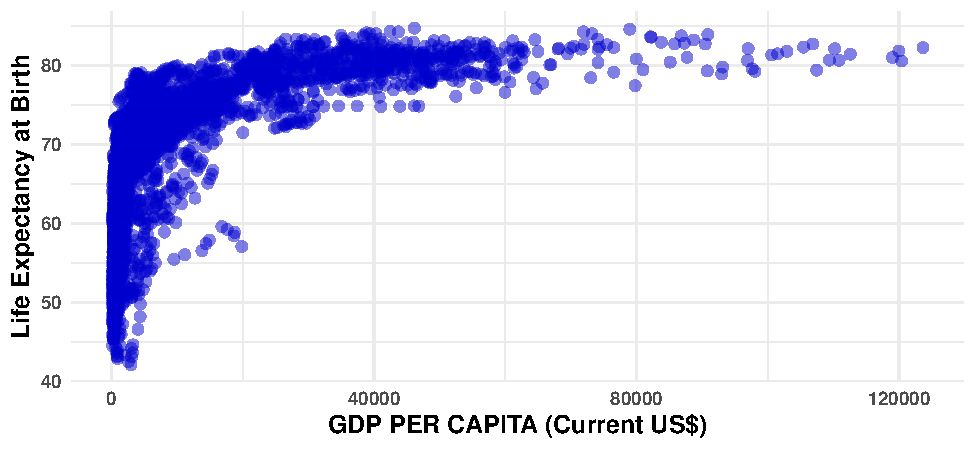
\includegraphics{Report_files/figure-latex/plot13-1.pdf}
\caption{GDP Vs Life Expectancy 2000-2017}
\end{figure}

Figure 13 shows the relationship between Life expectancy at birth vs GDP
per capita. In countries where the GDP is low life expectancy is also
low. As gradually the GDP per capita is increasing the life expectancy
is also increasing. We can see a major saturation at 40000 USD. But
after that one point, there is not much change in the life expectancy.
This may be because up to that point, all the basic necessities are
getting fulfilled but after that point, people are investing in luxeries
things which maybe irrelevant to the contribution in life expectancy. We
still see slight increase, that is maybe due to increase in population.

\begin{figure}
\centering
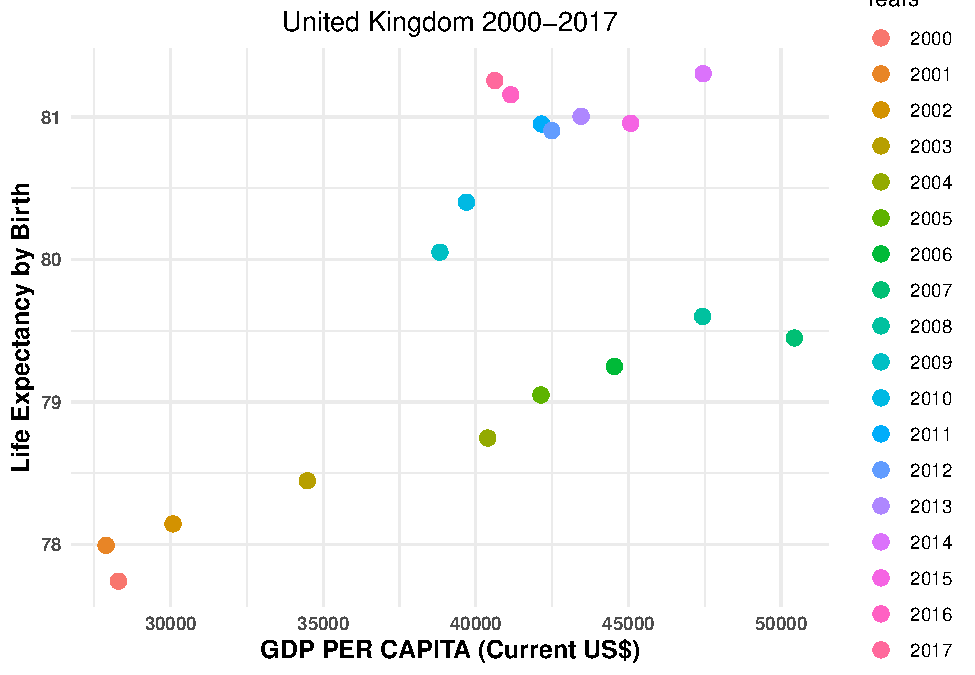
\includegraphics{Report_files/figure-latex/plot14-1.pdf}
\caption{GDP Vs Life Expectancy UK 2000-2017}
\end{figure}

Figure 14 shows a relationship between life expectancy and GDP in the
UK. We could see that as the years pass by life expectancy is
increasing. In 2016 the life expectancy value is around 81. We could see
a slight change in the behaviour in 2008. This may be because of the
Financial crisis in 2008. We can see the same behaviour as before after
a certain point there is not much change in the value similarly like we
saw in Figure 11. The life expectancy value gets stable.

\hypertarget{variation-of-the-relationship-across-different-countries-and-possible-correlation-with-historical-events-2000-2017-2}{%
\subsection{Variation of the relationship across different countries and
possible correlation with historical events (2000
--2017)}\label{variation-of-the-relationship-across-different-countries-and-possible-correlation-with-historical-events-2000-2017-2}}

\begin{figure}
\centering
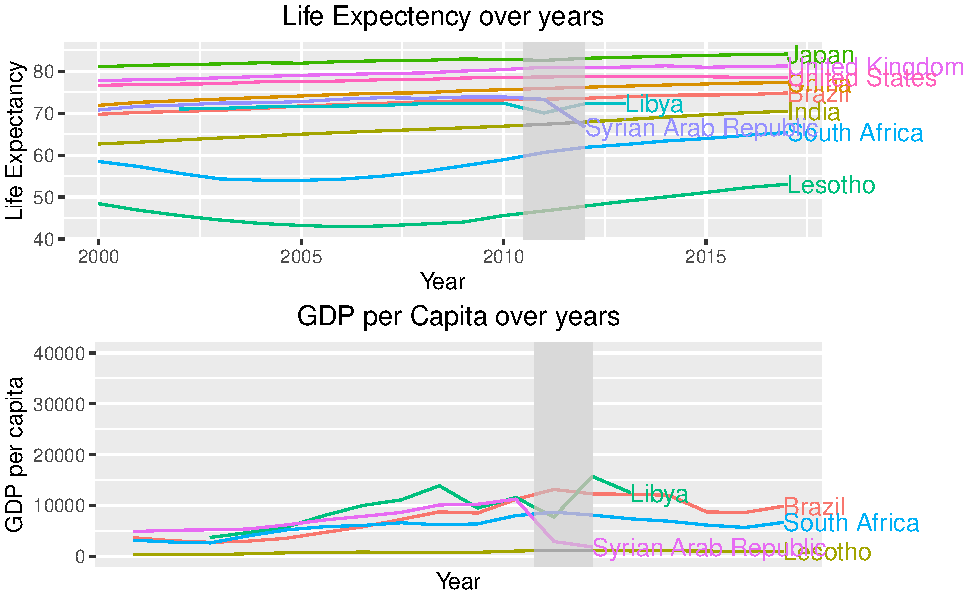
\includegraphics{Report_files/figure-latex/plot15-1.pdf}
\caption{Historic events in certain countries 2000-2017}
\end{figure}

From figure 15, we can make following observation:

\begin{itemize}
\tightlist
\item
  We can see a breakdown of life expectancy in the period 2011-2012 for
  Syria and Libya. This is likely due to the Civil war in Libya and
  Syria.
\item
  The impact on life expectancy is on a larger-scale in Syria as there
  was a high death toll which may result in a drastic decrease in life
  expectancy since the war was still going on ill the recent cease-fire
  agreement in 2021.
\item
  And that may be the reason we can there is no data from Syria after
  2012.
\item
  South Africa: Suffering from HIV/AIDS epidemic since 1995 may cause a
  drop in life expectancy to the lowest in 2005.
\item
  Same as South Africa, it can also be seen in Lesotho, potentially due
  to the same reason.
\end{itemize}

\hypertarget{gdp-per-capita-and-health-indicator-relationships-between-countries-over-time-2000-2017}{%
\subsection{GDP per capita and health indicator relationships between
countries over time (2000
--2017)}\label{gdp-per-capita-and-health-indicator-relationships-between-countries-over-time-2000-2017}}

\begin{figure}[H]

{\centering \includegraphics[width=1\linewidth]{./health_gdp_uk} 

}

\caption{Health Expenditure UK and world 2000-2017}\label{fig:plot16}
\end{figure}

In the above graph we see the relationship between Health expenditure
per capita and GDP. In the left graph in figure 16, we can see that
countries with lower GDP value have much less Health expenditure per
capita. We can see a linear growth in expenditure as the GDP increases.
But after a point, there is not much increase maybe because after that
point the government must be investing the money somewhere else. We can
see the highest to be 10000 where the GDP is 60000 USD. And the lowest
is at 0. In the right graph in figure 16 we see the relationship is only
of the UK. We can see a linear increase in the value of health
expenditure. The maximum is at 4500 in 2017. We can see a slight change
in the graph at 2008. This is caused because of the Financial crisis.

\hypertarget{assessing-causality-does-wealth-cause-health-or-vice-versa}{%
\subsection{Assessing causality: Does wealth cause health or vice
versa?}\label{assessing-causality-does-wealth-cause-health-or-vice-versa}}

As seen in Procedure section we get 2 models each for wealth and health
indicators as input and outputs, one with and one without confounding
factors. let's see the results.

\begin{figure}[H]

{\centering \includegraphics[width=0.6\linewidth]{./wealth_health} 

}

\caption{Health Expenditure UK and world 2000-2017}\label{fig:plot17}
\end{figure}

As we see the R-square value from the output snippet in figure 17 where
wealth indicators are input, the model without HDI values performed much
worse with R-square value of 0.38 which is a drastic drop in performance
as compare to model with HDI in it, although the GDP per capita seems
statistically significant as it ahs high coefficient magnitude and
\textless0.05 p-value. While this is not true when we have health
indicators as inputs, we observed that we got 0.78 with external balance
as input and 0.75 without external balance as confounding factor. The
result can be seen in figure 18.

\begin{figure}[H]

{\centering \includegraphics[width=0.8\linewidth]{./ext_model} 

}

\caption{Health Expenditure UK and world 2000-2017}\label{fig:plot18}
\end{figure}

\hypertarget{conclusions}{%
\section{Conclusions}\label{conclusions}}

In the results we have seen the impact of GDP per capita on multiple
health factors, and we got to see that for some indicators we see a
change upto certain value of GDP per capita while for some health
indicators like MMR the relationship seems independent. We have also
seen that presence of various historical events had major impact on
health factors as we see multiple breaks in various countries for these
indicators despite their GDP per capita increasing.

We also ran multiple regression model and found out that the certain
wealth factors we took were not a good fit for the health indicators,
although out of all the wealth indicators we took, we did found out that
GDP per capita was statistically significant, but after doing causality
assessment with the help of confounding factor we can conclude overall
wealth indicators including GDP per capita has less impact on health.
While on the other hand we see that health indicators were at least
significant to GDP per capita which is considered as one of the most
important economic indicator. Resulting in the conclusion that health
causes wealth.

\hypertarget{references}{%
\section*{References}\label{references}}
\addcontentsline{toc}{section}{References}

\hypertarget{refs}{}
\begin{CSLReferences}{1}{0}
\leavevmode\vadjust pre{\hypertarget{ref-Worlddata}{}}%
BANK, T.W. 2023. World bank open data. {[}Accessed 1 May 2023{]}.
Available from: \url{Https://data.worldbank.org/}.

\leavevmode\vadjust pre{\hypertarget{ref-who}{}}%
Organization, W.H. 2023. THE GLOBAL HEALTH OBSERVATORY. {[}Accessed 1
May 2023{]}. Available from:
\url{https://www.who.int/data/gho/indicator-metadata-registry/}.

\end{CSLReferences}

\end{document}
